\documentclass[main.tex]{subfiles}

\begin{document}
\chapter{Benchmarking and Literature Review}
\chaplabel{literatureReview}

\section{Benchmarking}

After undertaking a benchmarking process, as detailed in \Chapref{benchmarking}, several key challenges were identified in regards to the platform and landmine detection, namely signal processing, automation and navigation. In order to better understand the issues associated with these subjects, a literature review is conducted. This also serves to influence concept design selections. 

\section{Signal processing}
Signal processing is a major component for this project with the main aim to utilise the raw signal output from both a metal detector and a GPR to be processed into a format that is able to be used in the detection of landmines.  
\seclabel{splitreview}

\subsection{Metal detector signal processing}
A metal detector operates on a similar arrangement of equipment as a GPR unit, with both systems utilising a transmitting source and a receiving device to detect objects. Metal detectors that operate on the eddy current principle generate magnetic fields which penetrate the soil, inducing eddy currents in underground metallic objects. These eddy currents in turn generate a secondary magnetic field, at a greatly reduced amplitude, which can then be detected by the receiving coil of the metal detector \parencite{Candy2008}. Similar to the GPR, the signal to noise ratio is low, especially in heavily mineralised soils, and all signals are heavily attenuated with depth \parencite{Candy2008}.

Consumer-marketed metal detector devices convert the received signals directly to an audio signal, where an operator can distinguish metal objects from non-metals by the amplitude and tone of the received signal.  Using this method qualified demining personnel can readily locate the position of a subsurface object, however full classification of the object or determination of its characteristics, such as size, shape and material are practically impossible \parencite{Kruger2006}. Some degree of basic automatic classification is common on devices marketed for treasure hunting, where it is used to distinguish valuable metallic objects from common metals. This classification is known as a discriminated signal and is possible due to the variation in eddy currents induced by different metals - most particularly between ferrous and non-ferrous metals. 

The signal response that allows the creation of the discriminated signal is the time constant of the received audio sample. The time constant is a function of the metallic material being detected, based largely on the target inductance and conductivity \parencite{Candy2008}. Selectively discriminating times when the signal's time constant meets a certain criteria allows for the detection of different metal types, with most ferrous targets having very long time constants, and targets composed of other metals being able to be discriminated based on expected time constant range \parencite{Candy2008}. This method however is not generally applicable to the purposes of landmine detection as the size and shape of a material can influence the time constant, and as such the method is not reliable for typical landmines, which consist of small parts of different materials and complex shapes \parencite{Kruger2006}. The influence of mineralised soil is also not compensated for by the discriminator which would also affect the determination of metal type \parencite{Kruger2006}.

A method more appropriate for landmine detection, and particularly automatic landmine detection, is the generation of signatures of landmine objects from a sample of training data sets. A signature of an object can be generated from the phase loop representation of the sample signal in the complex plane, an advantageous strategy as the required signal to noise ratio for a quality signature is low \parencite{Kruger2006}. Example object signatures showing the variance between objects are shown in \Figref{signature}.
% Cut into separate pictures, subfig
\begin{figure}[ht]
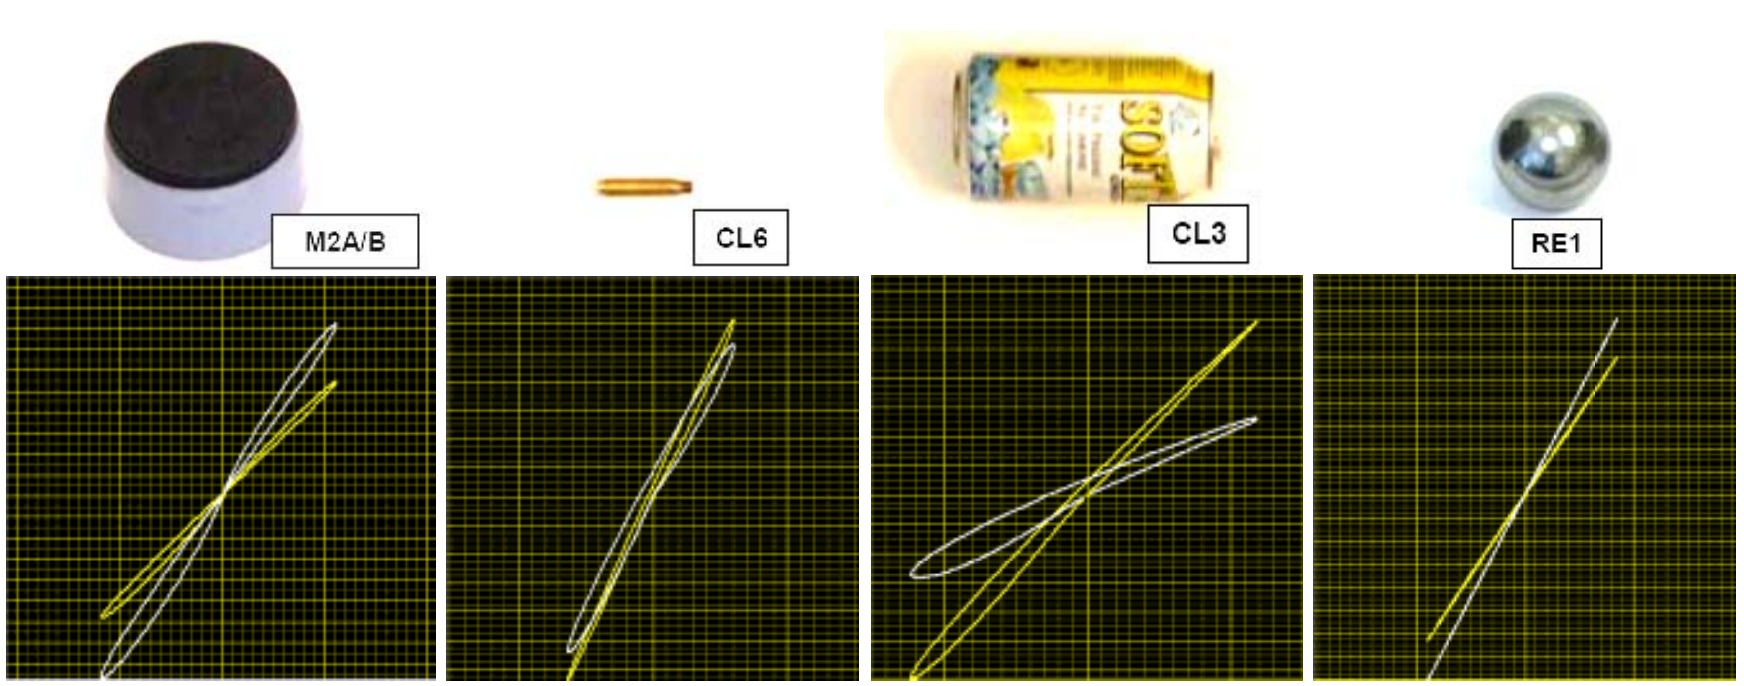
\includegraphics[width=0.8\textwidth]{2-LiteratureReview/signature.png}
\centering
\caption[Phase plot signatures of various potential subsurface objects]{Phase plot signatures of various potential subsurface objects - a landmine, bullet casing, soft drink can, steel ball (from left to right) \parencite{Kruger2006}} \figlabel{signature}
\end{figure}

This signature is capable of uniquely identifying an object type (to a certain degree) allowing comparison of detected samples against a limited set of known signatures, yielding an object classification. The low signal to noise ratio requirement also means that the strategy is reasonably robust against depth based attenuation, allowing consistent classification of objects irrespective of depth. This result is shown in \Figref{comp-signature}. \Figref{comp-signature} also highlights the requirement for ground signal compensation to allow for correct matching of signatures. The ground compensation process is similar to that described for GPR technology. Important to note is that the ground compensation algorithm used on the samples must be identical to the ground compensation algorithm used to generate the signatures from the training set to guarantee comparability \parencite{Kruger2006}.
\begin{figure}[ht]
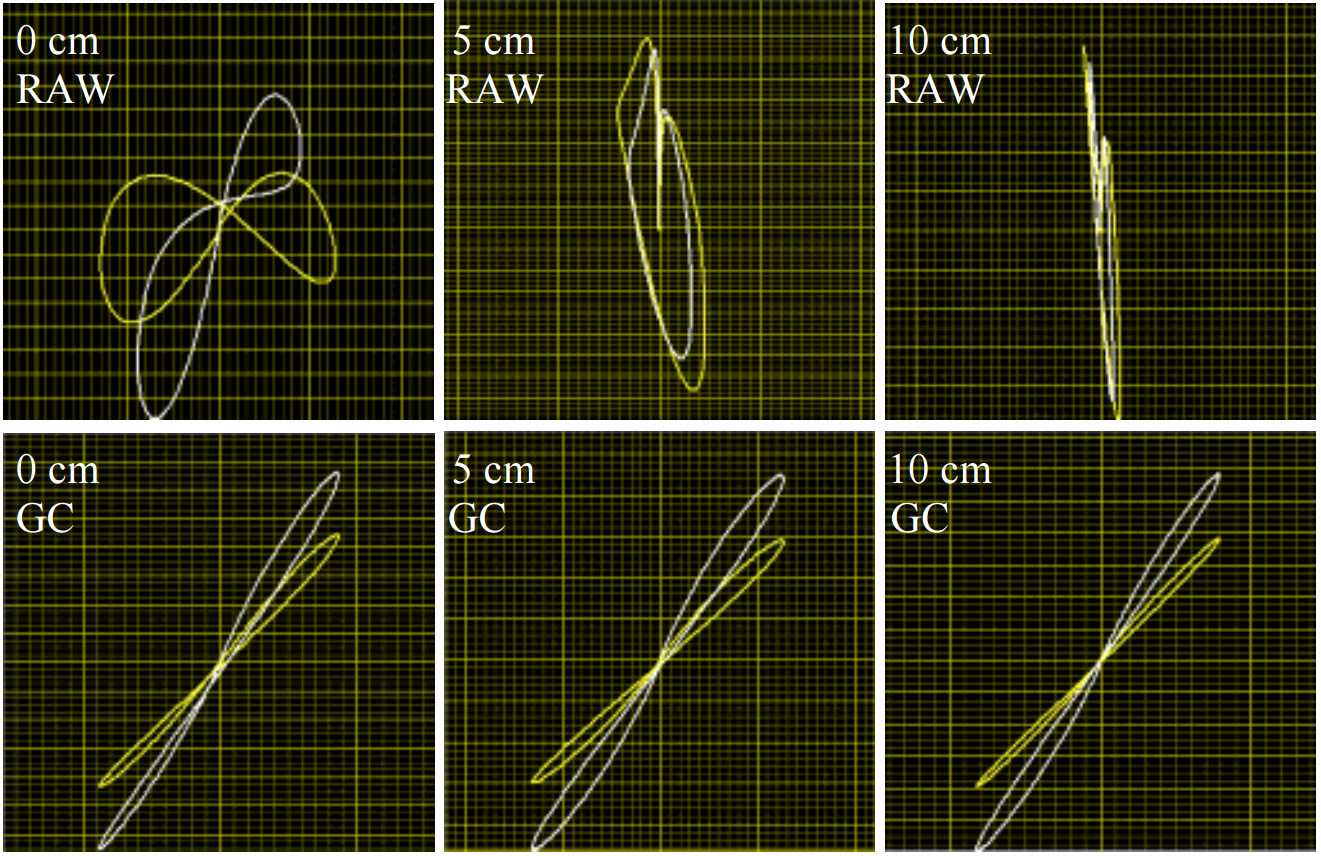
\includegraphics[width=0.8\textwidth]{2-LiteratureReview/compensated-signature.png}
\centering
\caption[Phase plot signatures of a landmine at varying depths]{Phase plot signatures of a landmine at varying depths. The top row shows the raw data phase plot and the bottom row shows the ground compensated signal \parencite{Kruger2006}} \figlabel{comp-signature}
\end{figure}

The signature method has a notable failure point where the presence of a metallic non-landmine object situated immediately next to a landmine can interfere with the signature of the received sample, reducing the likelihood that a correct identification will be made. This is particularly problematic where large metallic objects can completely obscure the signature of smaller objects. As a result, this technique is limited to situations in which metallic contamination is sparse, or metallic objects are typically an order of magnitude smaller than the objects of interest \parencite{Kruger2006}.

\subsection{GPR signal processing}
\seclabel{gpr}
\subsubsection{Hardware configuration influence on detection capability}
Ground Penetrating Radar operates by measuring reflected radio signals, caused by changes in density in underground materials, usually occurring at the interface between objects and the soil \parencite{sakaguchi2014}. Achieving a high signal to noise ratio is a challenge with GPR, as signal noise is introduced at all locations where even a small change in density occurs \parencite{shresta2003}. Thus, the primary challenge when searching for objects using GPR technology is being capable of distinguishing important objects from a noisy signal response \parencite{sakaguchi2014}.

Radar frequencies are attenuated by underground objects as they absorb the energy in the transmitting signal, dampening the possible response to the receiving antenna. This is particularly problematic in certain soil types, notably wet soils and clays, that have a significant damping effect on the radar pulses \parencite{sakaguchi2014}. Increasing the power of the transmitted signal or increasing the gain on the receiving signal both serve to reduce the effects of ground attenuation and allow for greater scanning depth with GPR \parencite{Ho2008}. The ability to increase both of these factors is limited by the capacities of the controlling electronics which, in turn, is limited by the state-of-the-art amplifier technologies. This places an effective limit on the scanning depth allowable with GPR technology. Increasing the receiver gain also has the affect of amplifying any noise generated through the system, making the ability to detect subsurface objects heavily constrained by the ability to differentiate objects of interest from non-significant features \parencite{shresta2003}. Due to the attenuation of the radar signal through the soil, and the limits on the receiving signal gain; a trade-off exists between the maximum sensing depth and the detection resolution \parencite{Ho2008}.

Wideband frequency coverage is a radar scanning strategy which can be used to achieve high resolution scanning and high depth capabilities, overcoming the limitations of the control electronics. As different frequencies experience different levels of attenuation, a lower frequency transmitter and receiver (200 MHz) will be capable of detecting at greater depths than a high frequency, at the sacrifice of detection resolution. Conversely high frequency systems ($\sim$3 GHz) will achieve greater resolution at the cost of severe attenuation with increased depth \parencite{shresta2003}. Wideband frequency coverage is the application of antennas which are capable of varying their frequency to allow a single device to scan over a wide frequency band. By collating detection results from multiple frequencies a combined response can be created, which has signal responses from large, deep objects while retaining the ability to distinguish small objects at shallow depths \parencite{3dradarDXG}.

A limitation restricting the application of GPR technology for the purposes of UXO scanning is the small search area. The detection of subsurface objects is effectively limited to objects situated between the transmitting and receiving antennas, which in practice must be only a small distance apart due to signal attenuation. This prevents the scanning of wide fields by placing the antennas a wide distance apart. Iterative scanning must be employed to cover a zone, and with a small scan width this requires a great number of scans.

The limitation of a single radar scanline has been overcome with the use of an array of transmitting and receiving antennas combined into a single scanning device. Under this arrangement the series of transmitting and receiving antennas are displaced laterally from each other along the length of the device, as shown in \Figref{arraylayout}. The application of multiple transmitting and receiving pairs allows for a single pass to scan a significant width, limited only by the number of transmitting and receiving pairs \parencite{3dradarDX}. The proximity of the transmitting pairs also allows for the signal difference at the receiving antennas to be interpreted from multiple transmitters, thereby greatly increasing the fidelity of the scan. The effective sensing locations by pairing each receive antenna to two transmitting antennas are shown as red dots in \Figref{arraylayout}. A scanning device of this kind would be far more costly than a radar system that was only capable of producing a single scanline.

\begin{figure}[ht]
\centering
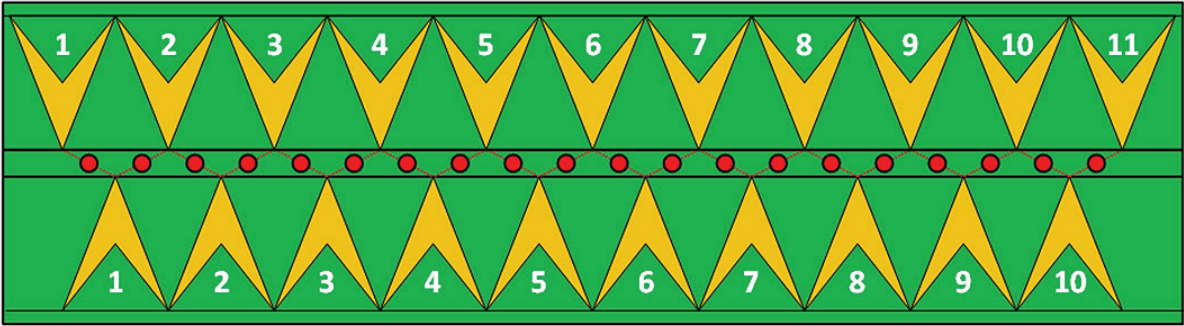
\includegraphics[width=0.8\textwidth]{2-LiteratureReview/3d-radar.png}
\caption[Example layout of transmitting and receiving elements of a 3D radar system]{Example layout of transmitting (bottom row) and receiving elements (top row) of a 3D radar system \parencite{3dradarDXG}}
\figlabel{arraylayout}
\end{figure}

\subsubsection{Signal processing and determination of objects of interest}
Typically the software processing flow for ground penetrating radars used for landmine detection purposes consists of preliminary preprocessing, which involves the background signal removal and clutter suppression; the initial detection, which involves selection of all suspicious anomalies present in the scan, and classification; the process of analysing the data and determining which of the suspicious anomalies have a high likelihood of being a landmine or other dangerous object \parencite{Ho.etal2004}. This process requires determining a set of classification characteristics which suitably and uniquely identify the feature of an object of interest. These characteristics are limited by those which can be accurately measured by the GPR device, and are commonly the size, shape and other physical aspects of the object \parencite{Ho2008}. However, objects can also be identified from the raw signal without the need to link parameters to real-world object characteristics, by identifying objects through particular patterns present in the time-frequency plane at the receiving antenna.

Detection of landmine responses with GPR data is made difficult by the low signal to noise ratio, making preliminary filtering difficult \parencite{shresta2003}. The largest noise component of the received signal is the response due to the air-ground interface, which generates a strong response and can obscure the features of objects of interest that only generate a small signal \parencite{Yarovoy2009}. As a result, minimal elevation of the GPR device is desirable as this minimises the influence of this air-ground interface reflection on the received data. Noise is further reduced from the received signal through statistical tests applied over successive scans, such as Kalman filters, artificial neural networks and fuzzy logic tests. These algorithms form the preprocessing stage of the processing chain described above.

The easiest way to detect an object is if the approximate response is previously known, such as from a model or training data set \parencite{Yarovoy2009}. Algorithms have been developed which identify pattern matches between a known expected response and the received response from the GPR. The most popular algorithm for this application is the inverse-matched filter, which is a mathematical convolution over the received signal to attempt to detect the presence of the expected response \parencite{Osumi1984}. More advanced algorithms are capable of producing results with greater accuracy when correlated with detection confidences from nearby samples. If a number of samples in a local area show high confidence in a detected object, the overall confidence that a detection has occurred increases when compared to an isolated positive detection. The hyperbola detection method attempts to identify the hyperbolic shape formed in a visual image when multiple samples are combined in this manner (as in \Figref{GPRsample}), through the use of computer vision techniques such as edge detection and the randomised Hough transform \parencite{Xu1990}.
\begin{figure}[ht]
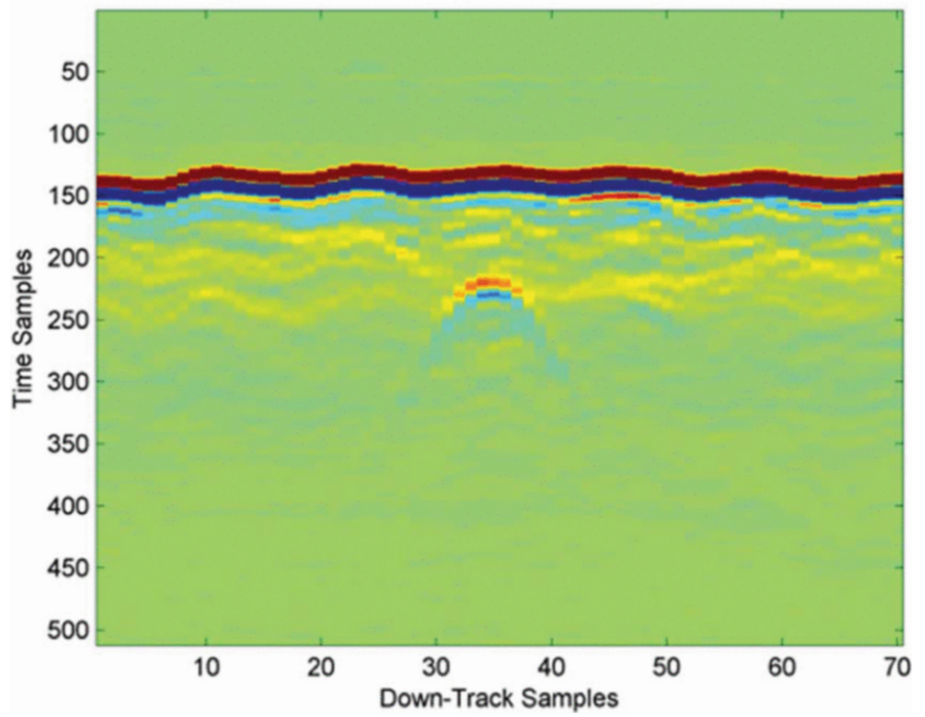
\includegraphics[width=0.7\textwidth]{2-LiteratureReview/GPR-sample.png}
\centering
\caption[Sample GPR response over buried anti-tank mine]{Sample GPR response over buried anti-tank mine showing parabolic shape in received signal over object of interest, which can be detected using the randomised Hough transform method} \figlabel{GPRsample}
\end{figure}

These algorithms represent the initial detection stage of the processing chain. Further classification of objects to reduce false-positive testing is possible through artificial intelligence strategies such as neural networks or decision trees, which require extensive sets of training data to produce strongly confident results, or through the pairing of the GPR detection with detection confirmation from a secondary sensor, such as a metal detector.

\section{Sensor fusion for landmine detection}
The wide range of potential materials, shapes and burial depths of dangerous underground objects and the constraints of sensing technologies means that single sensor based systems are limited in their detection capacity \parencite{Yarovoy2009}. Combination sensing allows access to a wider gamut of information about a particular subsurface object, allowing detection of a wider range of objects and heightened confidence in the detection rate of landmine and IEDs. Two potential configurations exist - where a single sensor is used as a primary detector with confirmation provided by secondary sensor, and where both sensors are used concurrently and information from both detectors is processed simultaneously. Mutual processing of the data from both sensors is called sensor fusion. A common distinction is made between potential levels of sensor fusion \parencite{Yarovoy2009}:
\begin{itemize}
\item \textbf{Decision-level fusion:} information from the sensors is evaluated individually and a decision is made (landmine or non-landmine) for each sensor. Confidence in the sensor's independent decision is compared against the decision vector to produce a final determination.
\item \textbf{Feature-level fusion:} information from the sensors is produced from the raw sensor data individually. This information is then combined from all sensors to create a singular feature, with a single and final determination made against this feature. 
\item \textbf{Data-level fusion:} data is combined from all sensors to produce a single set of information about the feature. A final determination is made against this feature.
\end{itemize}
Features are linked between sensors by associating samples across multiple sensors, generally by proximity. Features detected by different sensors within a certain threshold distance of each other are associated and considered as the same feature. Each progressive step down from decision-level fusion requires significantly greater computational processing, and greater knowledge of the sensor dynamics and the correlations of signal features to real-world object parameters \parencite{Yarovoy2009}. Higher level fusion strategies lend themselves well to machine learning techniques, which can be naive to the sensor mechanics and produce correlations based on learned sample data sets computationally cheaply. Experimental trials suggest that all forms of sensor fusion are capable of producing significantly more accurate detection results with far fewer false-positive incidents than single sensor systems \parencite{Yarovoy2009}.

\section{Automation and navigation}
\seclabel{navigationandautomation}
The challenges of the automation and navigation of the platform are identified and overcome through different methods of implementation. Autonomous control of the platform is implemented using PID control and fuzzy logic concepts by identifying the relevant input parameters for these methods. Autonomous navigation of the platform is implemented through different path tracking and turning methods.  

\subsection{Autonomous control of a platform}
\seclabel{autocontrol}
In order to overcome the challenges for autonomous navigation, the autonomous control of the platform is required to be implemented through different methods identified in similar projects \parencite{zhao2012design,scheiner2011}. The control of the platform requires the main functions: throttle, braking, steering and gears (where applicable) \parencite{zhao2012design}. In order to control these functions, the platform requires attachment of actuators, sensors or servo motors to read their relevant state (conditions): speed, acceleration, brake pressure, steering angle and gear change. These parameters are dependent on how the actuators and sensors work in conjunction with the functions of the platform. The throttle attached with a servo motor translates the wheel motion from a frequency to voltage, which is proportional to the acceleration \parencite{zhao2012design,scheiner2011}. This voltage state may be used to calculate the equivalent output speed in order to determine the voltage change required to achieve acceleration or deceleration of the platform \parencite{scheiner2011}.The orientation state of the platform is used as an input parameter for steering control where the steering angle is defined for each position and direction. Similar projects have implemented this analogy where the steering angle is calculated based on the changes to shaft (gears) revolutions and ratios in order to determine the platform orientation \parencite{zhang2010study,zhao2012design}. The brake controller is used to change the direction of the linear motor and, in turn, change the brake pressure \parencite{zhao2012design}. The gears are controlled in conjunction with the throttle to limit the output of the motor (speed) and change direction (forward and reverse) \parencite{tran2007modelling}.

The main approach used for control of these parameters is the PID controller \parencite{zhao2012design,tran2007modelling,johnson2005pid}. 
The PID control uses a feedback system where the difference between the expected and actual outcome (error) can then used as an input parameter to the PID controller \parencite{johnson2005pid}. The output (result) is adjusted and looped back to the input as shown in \Figref{PIDblock}. 

\begin{figure}[ht]
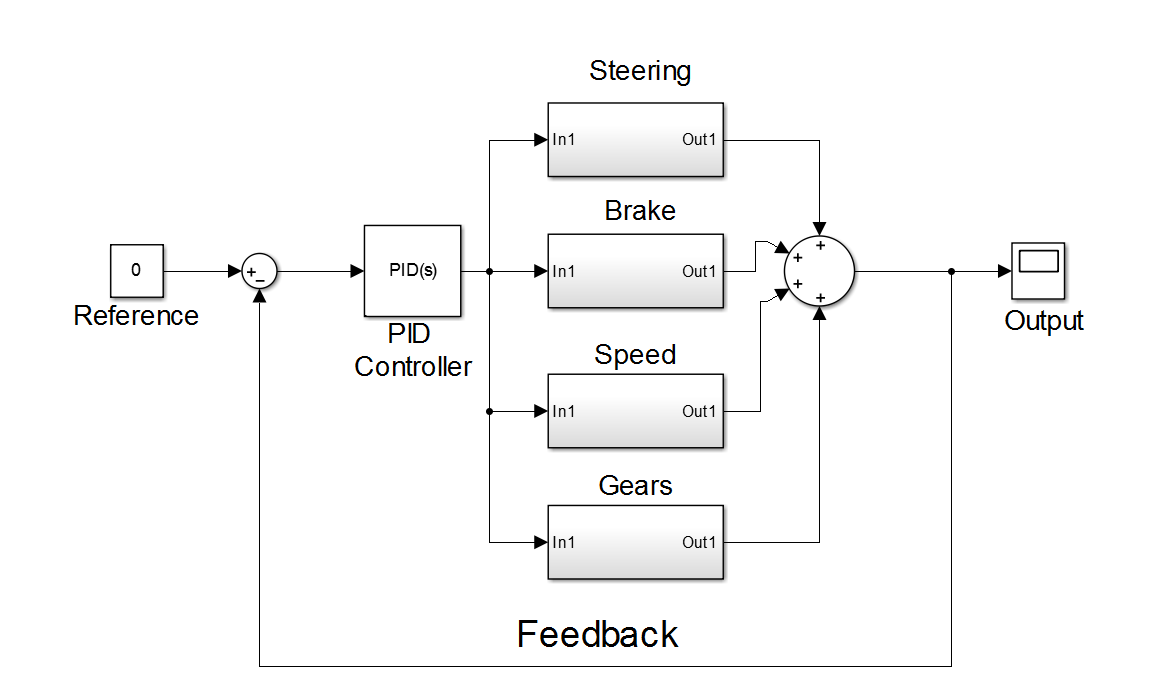
\includegraphics[width=\textwidth]{2-LiteratureReview/PIDblock.PNG}
\centering
\caption[PID controller block diagram for platform automation]{PID controller block diagram for platform automation\parencite{johnson2005pid}} 
\figlabel{PIDblock}
\end{figure}

An advantage of using the PID controller, as shown in \Figref{PIDblock}, is that it allows for single or multiple inputs, therefore, each function may have its own individual PID control loop or may be combined \parencite{johnson2005pid}. The latter is more difficult to achieve, however, the response from the inputs may be tuned automatically using a number of methods and implemented through software programs, such as, Matlab and Simulink, or other programming language libraries \parencite{tran2007modelling,johnson2005pid}. The challenge of implementing a  PID controller is that it is generally more complex due to the advanced mathematics required to determine the specific input parameters \parencite{tran2007modelling}. In addition, external inputs such as aerodynamics and relevant forces acted on the platform must be included in calculations as they change the expected outputs through the feedback loop of the controller \parencite{zhao2012design,johnson2005pid}. 

Another method for autonomous control of the vehicle is the implementation of fuzzy control in conjunction with the PID controller \parencite{zhang2009fuzzy}. The main (membership) functions will have its own logical variables for different levels of state (low, medium and high or slow, normal and fast)\parencite{johnson2005pid}. These levels will have an expected output range that will determine if a change in the one or more of the input parameters are necessary \parencite{johnson2005pid}. The main challenge to implement this method is similar to that of PID control, where advanced mathematics are used with the additional fuzzy logic parameters. These challenges are overcome through advanced mathematics software, such as, Matlab, however, the efficiency for the response is dependent on the processing power of the on-board platform system. 

The general concepts of the PID controller theory and fuzzy logic may be used to derive simpler methods for platform control \parencite{Ledin2003}. These concepts may be implemented through embedded control systems \parencite{Ledin2003}. The implementation requires a lower processing power in comparison to Matlab and other processor-heavy programs as it does not require advanced mathematics. As such, this method uses a more dynamic and flexible approach through relevant software design changes \parencite{Ledin2003}. This may be useful for systems that require flexibility in design or require time-efficient processes. 

%\textcolor{red}{the previous paragraph is too detailed i think and belongs more in detailed design once we have all the sensors and stuff, maybe something a lot shorter like whats in blue?: i might be wrong, so just ignore me if i am} 
%\textcolor{blue}{Relevant sensors and servo motors are used to directly control and read all aspects of a platforms physical functions and condition. The difference between a wanted value and the physical value (error) can then used as an input parameter to the PID controller.} 
%\textcolor{red}{I was just thinking it is required since I was thinking more along the lines of basic background of how each function works. Which isn't worded properly above, I know. But these are the challenges that we need to implement, so the actuators are helping to change the parameters of each control function, each one has individual parameters that are considered...  I was trying to make it lead into how the states can be changed using matlab and just simpler C++/Java stuff. Since in C++ and Java, these states can be changed easily. That sort of thing. }
%yup, whats above is far too specific i think. and i dont think you need to talk about each function individually (steering, throttle, etc.) just say that a function is controlled by actuators and needs to be able to be read so we know the state of it to define an error for hte PID controller.
%maybe it is alright, see what the others reckon. if everyone else is happy, im happy - harry

\subsection{Path tracking}
\seclabel{pathTrackingLitReview}
Path tracking uses location information from a GPS or some other positioning system to guide a vehicle along a pre-defined course. In theory the path can be defined as a continuous function but this is inefficient in practice. Instead, a path is discretised and defined by a series of points, called waypoints (shown in \Figref{pathDefining}). A path can either be described as lines connecting the waypoints or as a series of closely spaced waypoints. Due to the implementation of path tracking systems on digital devices the path description will be discretised at some point and so the definition has no impact on the application of the methods described below \parencite{Giesbrecht2005}.

\begin{figure}[htbp]
\centering
\subfloat[Continuous path]{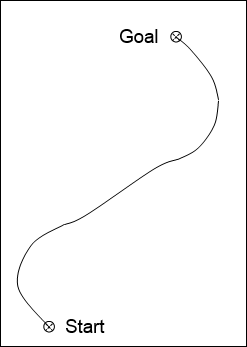
\includegraphics[width=0.28\textwidth]{2-LiteratureReview/pathContinuous.png}}\hspace{1em}%
\subfloat[Piecewise linear path]{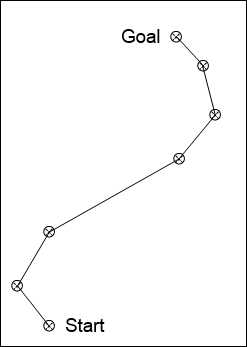
\includegraphics[width=0.28\textwidth]{2-LiteratureReview/pathPiecewise.png}}\hspace{1em}%
\subfloat[Set of discrete path nodes]{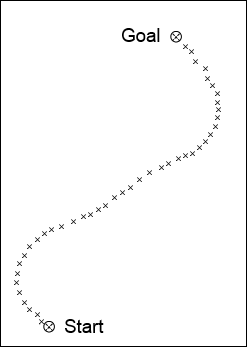
\includegraphics[width=0.28\textwidth]{2-LiteratureReview/pathDiscrete.png}}
\caption{Various ways to define a path \parencite{Giesbrecht2005}}
\figlabel{pathDefining}
\end{figure}

\subsubsection{Geometric path tracking}
Geometric path tracking uses geometric relationships between a vehicle and a path to produce a control algorithm as a solution to the problem. Theories assume vehicles use the Ackermann method for steering so a simplified steering model can be used for the geometry. This reveals a relationship between the steering angle and the curvature that the non steering wheels will follow. Two of the most commonly used geometric vehicle models are Pure Pursuit and the Stanley Method \parencite{snider2009}.

Pure Pursuit uses a path 'look-ahead' distance to measure the future error between the vehicle and the path in real time which can then be steered to and corrected for. \Figref{purePursuitGeom} shows the geometry associated with Pure Pursuit at one point in time. It shows a goal point $(g_x, g_y)$ on the desired path at a specified look-ahead distance $l_d$ in front of the vehicle. The steer angle is calculated based on an arc that would connect the centre of the non-steering axle to the goal point. The calculation of the goal point is effectively adding a waypoint to the path at that point. When high curvatures are present in a path the controller may begin to cut corners due to a look-ahead distance that would effectively skip this portion of the path. Lateral error on a path of constant curvature may also be experienced due to geometric controller characteristics which do not take into account the curvature of a path. However, Pure Pursuit provides a very robust tracking algorithm when discontinuous curvatures are present \parencite{snider2009}. In general, for more accurate tracking a short look-ahead distance should be used but will eventually result in oscillation, for smoother tracking a long look-ahead distance should be used but this will reduce precision \parencite{snider2009}.
\begin{figure}[ht]
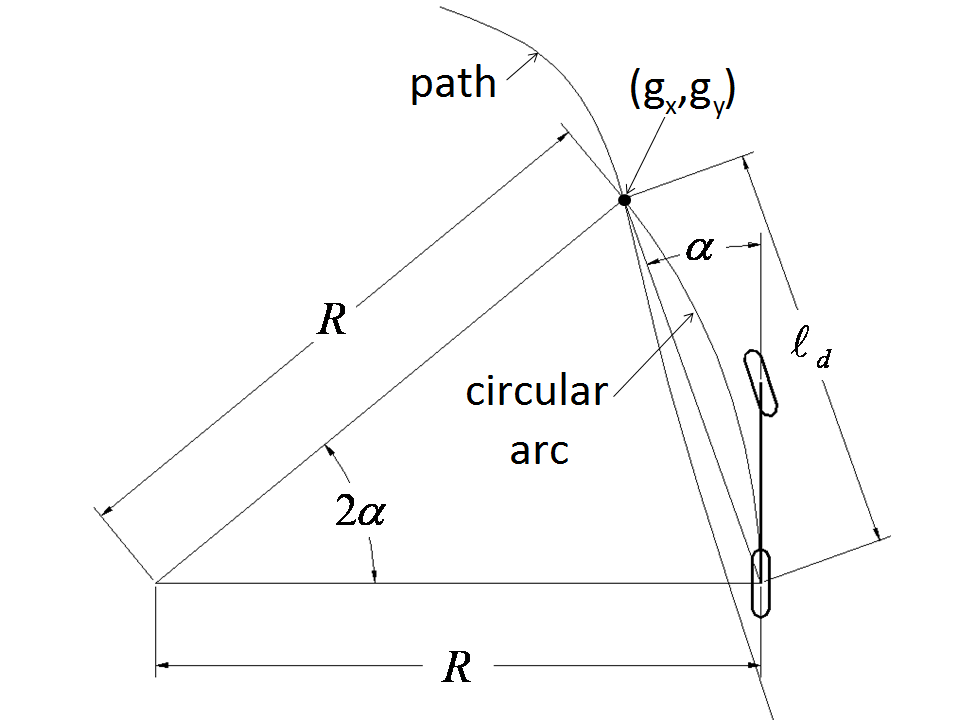
\includegraphics[width=0.6\textwidth]{2-LiteratureReview/purePursuitGoal.png}
\centering
\caption[Pure Pursuit geometry]{Pure Pursuit geometry \parencite{snider2009}} \figlabel{purePursuitGeom}
\end{figure}

The Stanley Model uses the lateral error between the centre of a wheels axle and the nearest path point (\Figref{stanleyGeom}). The desired effect is so that as the vehicle strays further from the path, the wheels steering angle is amplified in an attempt to correct for the error. The Stanley Method is very well suited to higher speed tracking but can run into problems when curvature discontinuities are present in the path. The model sets the steer angle to the heading error which is calculated as the difference between the vehicles heading and the instantaneous heading of the nearest point on the path, $\theta_e$. An extra term is used when the lateral error is non zero which amplifies the steer angle to a new value of $\delta$.
\begin{figure}[ht]
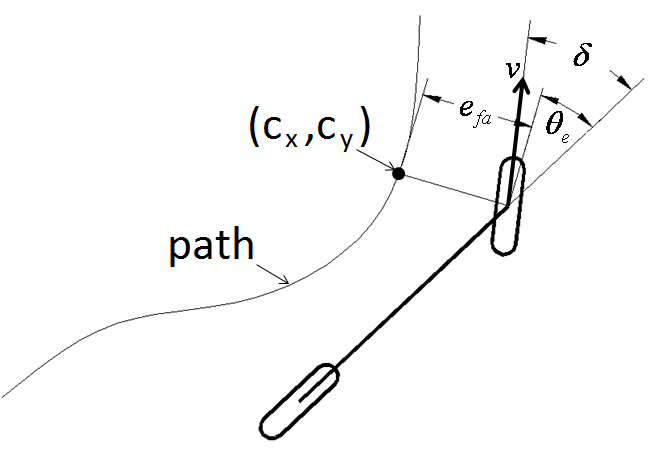
\includegraphics[width=0.5\textwidth]{2-LiteratureReview/stanleyMethod.png}
\centering
\caption[Stanley Method geometry]{Stanley Method geometry \parencite{snider2009}} \figlabel{stanleyGeom}
\end{figure}

Some limitations of geometric path tracking methods are related to the dynamics of a vehicle which are not present in the theory, namely the capabilities of a platform and its actuators. Due to this the method expects an instant response from elements such as the steering which is an issue when high path curvatures are present or when the curvature of the path suddenly changes. As a result the method cannot guarantee that the vehicle will follow a path as accurately as designed and at high speeds that vehicle may skid or tip \parencite{coulter1992}.

\subsubsection{Kinematic path tracking}
The kinematic model collapses a four wheeled vehicle into a two wheeled model, much like the geometric path tracking approach. The equations of motion for the simplified system are then used to relate the vehicle speed, change in heading error and change in lateral error to a user defined velocity and steer angle in path coordinates. In practice, the same trade off between performance and stability is apparent as in the geometric models, tracking accuracy declines at high speeds due to neglected dynamics \parencite{snider2009}. This method is not as robust as Pure Pursuit and displays a similar behaviour to the Stanley Method when discontinuities in curvature are present.
\subsubsection{Dynamic path tracking}
A dynamic model approximates the real dynamics of a vehicle which was one of the downfalls of the previous examples. Similar to the kinematic model, the vehicle speed, heading error and lateral error are related to a user defined velocity and steer angle in path coordinates. Even though the dynamics of the vehicle are included in this model, extreme path properties such as large changes in curvature can have a very large effect on the accuracy and efficiency of the path tracking \parencite{snider2009}. Discontinuities in the path still have a noticeable effect on accuracy and the steady state lateral error is still present. However, in a more realistic scenario a dynamic path tracking method does show overall improvement \parencite{snider2009}.

\subsection{Performing turning manoeuvres}
%maybe move this section to concept or detailed design AFTER we have established that our area subdivision is primarily linear. can then talk about it in more detail
In a path similar to that described by the piecewise linear definition, a turn can be moderately controlled by introducing a variable called the radial tolerance \parencite{Giesbrecht2005}. The radial tolerance describes the distance from the waypoint at which the system considers that waypoint 'reached', ultimately changing the point at which the platform will begin the turn towards the proceeding waypoint. If the radial tolerance is set too large the platform will begin the turn early resulting in poor path tracking. If the radial tolerance is set too small the platform will overshoot the desired path due to unaccounted vehicle dynamics and/or restrictions in steering angle. \Figref{waypointTolerances} shows examples of a radial tolerance set slightly too low (1 metre) in blue and more realistically in grey (6 metres) for a vehicle following the path in red with a turn radius of 4 metres. It is easily visible that both methods are unable to follow the desired path with perfect precision due to real vehicle dynamics.
\begin{figure}[ht]
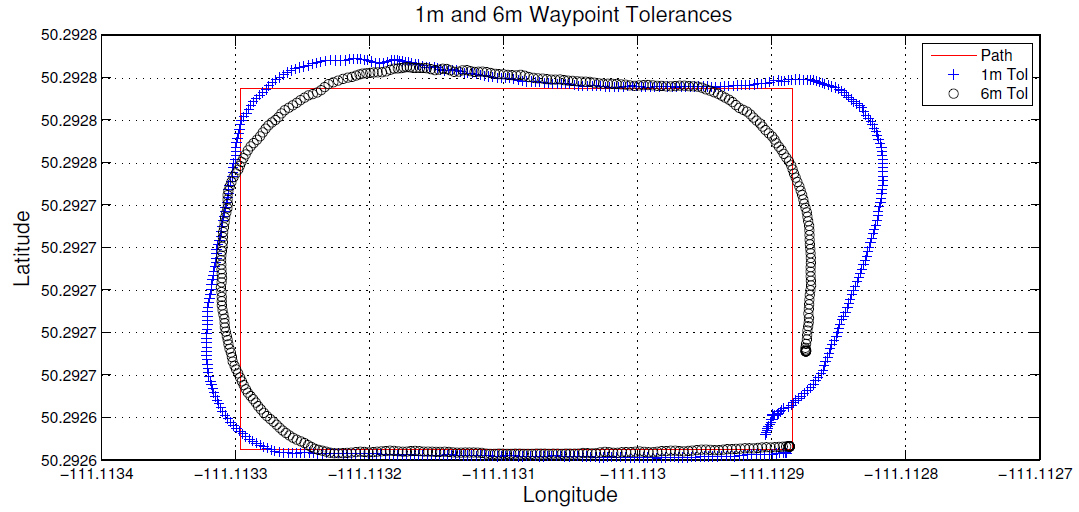
\includegraphics[width=\textwidth]{2-LiteratureReview/waypointTolerances.PNG}
\centering
\caption[Effect of waypoint tolerances on path tracking]{Effect of waypoint tolerances on path tracking \parencite{Giesbrecht2005}} \figlabel{waypointTolerances}
\end{figure}

\end{document}